\section{Hệ thống Chức năng Cốt lõi}

\subsection{Quản lý Phòng và Định tuyến Thông điệp}

\begin{enumerate}
    \item Cơ sở lý thuyết về Định tuyến Thông điệp và Mẫu thiết kế Xuất bản - Đăng ký (Publish-Subscribe)
    
    Trong hệ thống phân tán đa người dùng (Multi-user Distributed Systems), quá trình quản lý và phân phối thông điệp đòi hỏi các kỹ thuật kiểm soát tương tranh tài nguyên và tối ưu hóa định tuyến. Mẫu thiết kế Xuất bản - Đăng ký (Publish-Subscribe Pattern) được triển khai nhằm đáp ứng yêu cầu này. Trong đó, mỗi phòng trò chuyện (Chat Room) đóng vai trò tương đương một Chủ đề (Topic/Channel). Thực thể gửi (Publisher) đẩy thông điệp vào kênh, hệ thống tiến hành sao chép và phân phối thông điệp đến toàn bộ các thành viên đã đăng ký (Subscribers).
    
    Nhằm duy trì tính nhất quán dữ liệu (Data Consistency) trong môi trường truy cập đồng thời, hệ thống áp dụng cơ chế Khóa Đọc-Ghi (Reader-Writer Lock). Cơ cấu này cho phép các tiến trình đọc (Broadcast) thực thi song song theo mô hình phi chặn (Non-blocking), đồng thời cấp quyền truy xuất độc quyền cho các tiến trình ghi (Join/Leave/Create) nhằm ngăn ngừa hiện tượng tương tranh (Race Condition). Bên cạnh đó, quá trình thanh lọc dữ liệu (String Sanitization) được tích hợp tại điểm tiếp nhận nhằm giảm thiểu rủi ro từ các lỗ hổng tiêm nhiễm (XSS, SQL Injection).

    \item Triển khai Định tuyến và Quản lý phòng trong mã nguồn \\
% REMOVED BLANK LINE
    Hệ thống hiện thực hóa mô hình Pub/Sub thông qua lớp lõi \texttt{RoomManager}. Luồng dữ liệu trò chuyện \texttt{MSG\_CHAT\_SEND} được xử lý theo cấu trúc ba tầng:
    
    \begin{itemize}[label={-}]
        \item Tầng 1: Lọc dữ liệu (Detection \& Filtering): Khi tiếp nhận Payload, chuỗi \texttt{message} được xử lý qua phân hệ \texttt{MessageFilter}. Biểu thức chính quy (Regex) được triển khai nhằm nhận diện các mẫu dữ liệu không hợp lệ (XSS, SQLi). Trong trường hợp phát hiện vi phạm, hệ thống tiến hành loại bỏ toàn bộ thông điệp và lưu vết sự kiện vào AuditLog. Cơ chế này hoạt động theo mô hình phi trạng thái (Stateless).
        
        \item Tầng 2: Định tuyến và Phân phối (Routing \& Distribution): Hệ thống phân nhánh quy trình xử lý dựa trên loại hình thông điệp:
        \begin{itemize}[label={$\circ$}]
            \item Direct Message (Tin nhắn cá nhân): Tra cứu \texttt{ClientSession} của người nhận thông qua định danh bộ mô tả tệp (\texttt{fd}) và chuyển tiếp gói tin JSON.
            \item Room Message (Tin nhắn nhóm): Hàm \texttt{RoomManager::broadcastToRoom()} áp dụng khóa đọc \texttt{std::shared\_lock} để truy xuất danh sách thành viên (\texttt{members}) thuộc đối tượng \texttt{Room}. Hệ thống định tuyến thông điệp tới các \texttt{fd} đích qua hàm \texttt{ClientSession::sendPacket()}, ngoại trừ \texttt{excludeFd} (thực thể gửi).
        \end{itemize}
        
        \item Tầng 3: Lưu trữ và Đồng bộ (Persistence): Mỗi thực thể \texttt{Room} được ánh xạ 1-1 với đối tượng \texttt{ChatHistory}. Hàm \texttt{RoomManager::appendHistory()} lưu trữ tin nhắn vào cơ sở dữ liệu SQLite thông qua cơ chế Write-Ahead Logging (WAL). Khi máy khách yêu cầu tham gia phòng, tiến trình \texttt{sendHistoryToClient()} truy xuất $N$ bản ghi gần nhất và truyền tải nhằm đồng bộ ngữ cảnh.
        
        \item Cơ chế Quản lý Vòng đời (Lifecycle Management): Bảng \ref{tab:room_locks} đặc tả chiến lược quản lý tương tranh (Concurrency Strategy) trên biến \texttt{m\_mutex} của \texttt{RoomManager}. Cơ chế thu gom rác (Garbage Collection) được tích hợp tại hàm \texttt{leaveRoom()}, đảm nhiệm việc tự động giải phóng đối tượng \texttt{Room} và \texttt{ChatHistory} khi điều kiện \texttt{getMemberCount() == 0} thỏa mãn (ngoại trừ phòng mặc định).
    \end{itemize}
\end{enumerate}

\begin{longtable}{
    >{\raggedright\arraybackslash}p{4cm}
    >{\raggedright\arraybackslash}p{4cm}
    >{\raggedright\arraybackslash}p{6cm}
}
    \caption[Chiến lược cấp phát khóa trong RoomManager]{Chiến lược cấp phát khóa (Locking) trong RoomManager} \label{tab:room_locks} \\
    \toprule
    \multicolumn{1}{c}{\textbf{Tên Hàm (Method)}} & \multicolumn{1}{c}{\textbf{Loại Khóa (Lock Type)}} & \multicolumn{1}{c}{\textbf{Mục đích Kỹ thuật}} \\
    \midrule
    \endfirsthead
    
    \toprule
    \multicolumn{1}{c}{\textbf{Tên Hàm (Method)}} & \multicolumn{1}{c}{\textbf{Loại Khóa (Lock Type)}} & \multicolumn{1}{c}{\textbf{Mục đích Kỹ thuật}} \\
    \midrule
    \endhead
    
    \bottomrule
    \endfoot
    
    \bottomrule
    \endlastfoot

    \texttt{broadcastToRoom()} \newline \texttt{getUsersInRoom()} \newline \texttt{getRoomList()} & \texttt{std::shared\_lock} \newline (Khóa Đọc) & Hỗ trợ tiến trình phân phối thông điệp và truy xuất danh sách thực thi song song, duy trì cơ chế phi chặn (Non-blocking). \\

    \texttt{createRoom()} \newline \texttt{deleteRoom()} & \texttt{std::unique\_lock} \newline (Khóa Ghi) & Cấp quyền truy xuất độc quyền nhằm điều chỉnh cấu trúc \texttt{m\_rooms} và \texttt{m\_histories}, duy trì tính toàn vẹn cấu trúc (Structural Integrity). \\

    \texttt{joinRoom()} \newline \texttt{leaveRoom()} \newline \texttt{removeUser()} & \texttt{std::unique\_lock} \newline (Khóa Ghi) & Ngăn ngừa hiện tượng tương tranh trong quá trình cập nhật trạng thái \texttt{members} và cấu trúc ánh xạ \texttt{m\_fdToRoom}. \\
\end{longtable}

\begin{figure}[htbp]
    \centering
    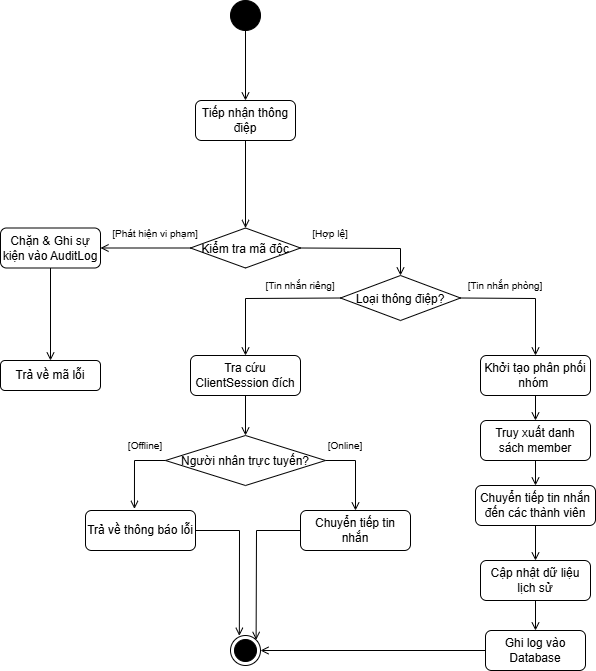
\includegraphics[width=0.65\textwidth]{Hinhve/hinh_2.5.png}
    \caption[Sơ đồ Hoạt động Định tuyến Thông điệp và Quản lý Phòng]{Sơ đồ Hoạt động Định tuyến Thông điệp và Quản lý Phòng}
    \label{fig:room_manager}
\end{figure}

\subsection{Trung chuyển Tệp tin Ẩn danh}

\begin{enumerate}
    \item Cơ sở lý thuyết về Kiến trúc Trung chuyển Ẩn danh \\
% REMOVED BLANK LINE
    Trong mô hình giao tiếp điểm-điểm (Peer-to-Peer - P2P) truyền thống, việc thiết lập kết nối trực tiếp giữa các thiết bị đầu cuối thường làm lộ địa chỉ IP thực. Đặc tính này làm gia tăng nguy cơ xâm phạm quyền riêng tư và tiềm ẩn rủi ro từ các cuộc tấn công từ chối dịch vụ (DDoS) hoặc truy vết danh tính (Doxing). 
    
    Hệ thống triển khai mô hình Trung chuyển qua Máy chủ (Server-Relayed Architecture) kết hợp cơ chế Phễu Proxy (Proxy Funneling). Máy chủ đóng vai trò trung gian, tiếp nhận các phân mảnh dữ liệu (Chunks) từ thực thể gửi và định tuyến trực tiếp tới thực thể nhận. Giải pháp này đảm bảo tính ẩn danh (Anonymity) thông qua việc che giấu địa chỉ IP đầu cuối. Đặc biệt, hệ thống ứng dụng kỹ thuật Đệm bộ nhớ tạm thời (In-Memory Buffering / Zero-Disk I/O) thay thế cho phương pháp lưu trữ - chuyển tiếp (Store-and-Forward) truyền thống, qua đó tối ưu hóa độ trễ I/O đĩa và loại trừ rủi ro cạn kiệt dung lượng lưu trữ của máy chủ.

    \item Triển khai Luồng Truyền tệp trong mã nguồn \\
% REMOVED BLANK LINE
    Lớp tĩnh \texttt{FileTransfer} điều phối quá trình xử lý tệp tin. Vòng đời phiên truyền tệp hoạt động dựa trên mô hình Máy trạng thái hữu hạn (Finite State Machine - FSM) gồm 4 pha:
    
    \begin{itemize}[label={-}]
        \item Pha 1 - Yêu cầu và Xác thực (PENDING): Khi tiếp nhận gói tin \texttt{MSG\_FILE\_REQUEST}, hệ thống cấp phát mã định danh \texttt{tid} (Transfer ID) thông qua bộ tạo số ngẫu nhiên an toàn CSPRNG. Hàm \texttt{isAllowedExtension()} thực thi kiểm duyệt định dạng tệp (hỗ trợ các định dạng: \texttt{.txt}, \texttt{.png}, \texttt{.jpg}, \texttt{.pdf}) và giới hạn dung lượng tối đa ở mức 3MB. Trong trường hợp hợp lệ, cấu trúc \texttt{FileTransferSession} được khởi tạo trên bộ nhớ, đồng thời lưu trữ mã băm SHA-256 nhằm hỗ trợ quá trình xác thực tính toàn vẹn ở cấp độ đầu cuối (End-to-End).
        
        \item Pha 2 - Phản hồi (ACCEPTED / REJECTED): Thực thể nhận tiến hành xử lý yêu cầu. Thông điệp từ chối (\texttt{MSG\_FILE\_REJECT}) sẽ kích hoạt quy trình hủy bỏ phiên giao dịch. Ngược lại, thông điệp chấp thuận (\texttt{MSG\_FILE\_ACCEPT}) sẽ chuyển trạng thái hệ thống sang \texttt{ACCEPTED}, qua đó thiết lập luồng truyền tải dữ liệu.
        
        \item Pha 3 - Trung chuyển dữ liệu (IN\_PROGRESS): Thực thể gửi tiến hành phân mảnh tệp thành các khối dữ liệu (Chunks) và tuần tự truyền tải thông qua gói tin \texttt{MSG\_FILE\_DATA}. Tiến trình \texttt{FileTransfer::handleData()} thực thi đối chiếu định danh \texttt{senderFd} nhằm mục đích xác thực, sau đó định tuyến (Relay) trực tiếp luồng tải trọng tới thực thể nhận \texttt{receiverFd}.
        
        \item Pha 4 - Hoàn tất và Thu hồi tài nguyên (COMPLETE / Garbage Collection): Thông điệp \texttt{MSG\_FILE\_COMPLETE} kích hoạt chức năng lưu vết hệ thống vào AuditLog và giải phóng phiên giao dịch. Đối với các phiên bị gián đoạn, tiến trình \texttt{cleanupExpired()} được kích hoạt định kỳ nhằm tự động thu hồi các giao dịch vượt quá giới hạn thời gian \texttt{TIMEOUT\_SEC}.
    \end{itemize}
\end{enumerate}

Bảng \ref{tab:file_states} tổng hợp các Trạng thái trong vòng đời của \texttt{FileTransferSession}.

\begin{longtable}{
    >{\raggedright\arraybackslash}p{3cm}
    >{\raggedright\arraybackslash}p{4cm}
    >{\raggedright\arraybackslash}p{7cm}
}
    \caption[Các trạng thái của Phiên truyền tệp]{Các trạng thái của Phiên truyền tệp (FileTransferSession)} \label{tab:file_states} \\
    \toprule
    \multicolumn{1}{c}{\textbf{Trạng thái (State)}} & \multicolumn{1}{c}{\textbf{Gói tin Kích hoạt}} & \multicolumn{1}{c}{\textbf{Mô tả Nghiệp vụ}} \\
    \midrule
    \endfirsthead
    
    \toprule
    \multicolumn{1}{c}{\textbf{Trạng thái (State)}} & \multicolumn{1}{c}{\textbf{Gói tin Kích hoạt}} & \multicolumn{1}{c}{\textbf{Mô tả Nghiệp vụ}} \\
    \midrule
    \endhead
    
    \bottomrule
    \endfoot
    
    \bottomrule
    \endlastfoot

    \texttt{PENDING} & \texttt{MSG\_FILE\_REQUEST} & Trạng thái chờ tín hiệu phản hồi từ thực thể nhận. Luồng dữ liệu truyền tải tạm thời bị phong tỏa. \\

    \texttt{ACCEPTED} & \texttt{MSG\_FILE\_ACCEPT} & Thực thể nhận chấp thuận giao dịch. Kích hoạt tiến trình tiếp nhận luồng dữ liệu (Data Chunks). \\

    \texttt{IN\_PROGRESS} & \texttt{MSG\_FILE\_DATA} & Tiến trình trung chuyển các khối dữ liệu (Chunks) giữa các thực thể. \\

    \texttt{(Destroyed)} & \texttt{MSG\_FILE\_COMPLETE} \newline \texttt{MSG\_FILE\_REJECT} & Phiên giao dịch bị thu hồi từ bộ nhớ hệ thống. Kết thúc vòng đời chuyển tiếp. \\
\end{longtable}

\begin{figure}[htbp]
    \centering
    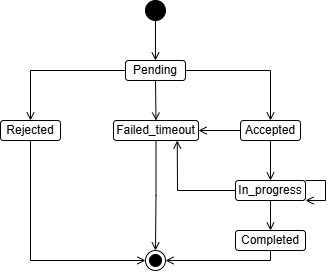
\includegraphics[width=0.55\textwidth]{Hinhve/hinh_2.6.png}
    \caption[Máy trạng thái hữu hạn luồng Truyền tệp ẩn danh]{Máy trạng thái hữu hạn (FSM) luồng Truyền tệp ẩn danh}
    \label{fig:file_transfer}
\end{figure}
